\frame{
\begin{center}
Applications of numerical techniques in science and engineering often involve {\Huge curve fitting}\footnote{曲线拟合} of experimental data. 
\end{center}
}

\frame{
\begin{block}{For example}
 in $1601$ the German astronomer Johannes Kepler formulated the third law of planetary motion\footnote{第三行星运动定律}, $T = Cx^{3/2}$, where
\begin{itemize}
\item  $x$ is the distance to the sun measured in millions of kilometers, 
\item $T$ is the orbital period measured in days, 
\item $C$ is a constant. 
\end{itemize}
\end{block}
\begin{center}
$\Downarrow$
\end{center}
\begin{block}{Problem "}
{\Large How to get the constant $C$}
\end{block}
}

\frame{
\begin{block}{ }
The observed data pairs $(x, T)$ for the first four planets, Mercury, Venus, Earth, and Mars\footnote{水星,金星,地球,火星}, are $(58, 88)$, $(108, 225)$, $(150, 365)$, and $(228, 687)$, and the coefficient $C$ obtained from {\Large the method of  least squares} is $C = 0.199769$. 
\end{block}
\begin{block}{The curve $T = 0.199769x^{3/2}$ and the data points are shown in following figure.} 
\begin{figure}
\begin{center}
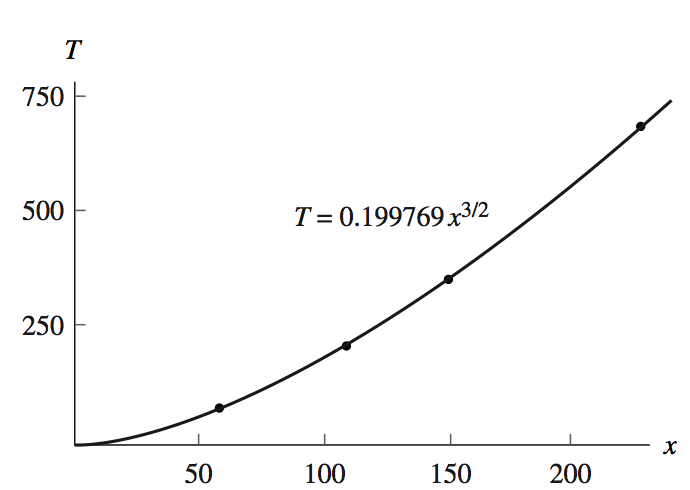
\includegraphics[width=50mm]{chap-4/fig_5-1.png}
\end{center}
\end{figure}
\end{block}
}
